%%% Template originaly created by Karol Kozioł (mail@karol-koziol.net) and modified for ShareLaTeX use

\documentclass[a4paper,11pt]{article}

\usepackage[T1]{fontenc}
\usepackage[utf8]{inputenc}
\usepackage{graphicx}
\usepackage{xcolor}
\usepackage[export]{adjustbox}
\usepackage{titlesec}
\usepackage{sectsty}
\allsectionsfont{\sffamily}
\usepackage{microtype}
\usepackage{tgheros}
\usepackage{droidsansmono}
\usepackage{mathptmx}
\usepackage{lastpage}
\usepackage{amsmath,amssymb,amsthm,textcomp}
\usepackage{enumerate}
\usepackage{multicol}
\usepackage{tikz}
\usepackage{tabto}
\usepackage{pxfonts}
\usepackage{geometry}
\geometry{left=25mm,right=25mm,%
bindingoffset=0mm, top=20mm,bottom=20mm}


\linespread{1.2}
\makeatletter
\renewcommand\tableofcontents{%
    \section*{\makebox[\linewidth][c]{\contentsname}%
      \@mkboth{\MakeUppercase\contentsname}{\MakeUppercase\contentsname}}%
    \begin{multicols}{2}%
    \@starttoc{toc}%
    \end{multicols}
    }
\makeatother
\newcommand{\linia}{\rule{\linewidth}{0.5pt}}

% custom theorems if needed
\newtheoremstyle{mytheor}
    {1ex}{1ex}{\normalfont}{0pt}{\scshape}{.}{1ex}
    {{\thmname{#1 }}{\thmnumber{#2}}{\thmnote{ (#3)}}}

\theoremstyle{mytheor}
\newtheorem{defi}{Definition}
\newtheoremstyle{mytheor}
    {1ex}{1ex}{\normalfont}{0pt}{\scshape}{|}{1ex}
    {{\thmname{#1 }}{}{\thmnote{ (#3)}}}

\theoremstyle{mytheor}
\newtheorem{nb}{Please Note}
% my own titles
\makeatletter
\renewcommand{\maketitle}{
\begin{center}
\vspace{2ex}
{\huge \textsf{\textbf{\@title}}}
\vspace{1ex}
\\
\linia\\
\textsf{\@date \hfill
\@author}
\vspace{4ex}
\end{center}
}
\makeatother
%%%
\usepackage{array}

% custom footers and headers
\usepackage{fancyhdr}
\pagestyle{fancy}
\lhead{}
\chead{}
\rhead{}
\lfoot{Assignment 6}
\cfoot{}
\rfoot{Page \thepage \ of \pageref{LastPage}}
\renewcommand{\headrulewidth}{0pt}
\renewcommand{\footrulewidth}{0pt}
%

% code listing settings
\usepackage{listings}
\usepackage[space=true]{accsupp}
\newcommand{\noncopynumber}[1]{
    \BeginAccSupp{method=escape,ActualText={}}
    #1
    \EndAccSupp{}
}
\definecolor{codegreen}{rgb}{0,0.6,0}
\definecolor{codegray}{rgb}{0.5,0.5,0.5}
\definecolor{inlinecode}{rgb}{0.1,0.1,0.1}
\definecolor{codepurple}{rgb}{0.58,0,0.82}
\definecolor{backcolour}{rgb}{0.95,0.95,0.92}
\lstset{
    language=C,
    basicstyle=\ttfamily\small,
    aboveskip={1.0\baselineskip},
    breakatwhitespace=false,         
    keepspaces=true,
    belowskip={1.0\baselineskip},
    columns=fullflexible,
    extendedchars=true,
    breaklines=true,
    tabsize=4,
    frame=lines,
    showtabs=false,
    showspaces=false,
    showstringspaces=false,
    commentstyle=\color{codegray},
    keywordstyle=\bfseries,
    %stringstyle=\rmfamily,
    numbers=left,
    numberstyle=\color{codegray}\footnotesize\noncopynumber,
    stepnumber=1,
    numbersep=10pt,
    captionpos=t,
    escapeinside={\%*}{*)},
}


\lstdefinestyle{output}{
    basicstyle=\ttfamily\small,
    aboveskip={1.0\baselineskip},
    breakatwhitespace=false,         
    keepspaces=true,
    belowskip={1.0\baselineskip},
    columns=fullflexible,
    extendedchars=true,
    breaklines=true,
    tabsize=4,
    frame=lines,
    showtabs=false,
    showspaces=false,
    showstringspaces=false,
    captionpos=t
}
%%%----------%%%----------%%%----------%%%----------%%%

\begin{document}

\title{CSE-016 Programming Lab Assignment \textnumero{} 6}

\date{17/05/2024}

\author{Youssef Ahmed Samy Kassem\\ \hfill ID 9545 -- Group 3 -- Lab 1\\ \hfill SSP -- Faculty of Engineering, Alexandria University\\}

\maketitle
\textsf{\textsl{\textbf{Solutions begin from the second page.\\Screenshots of console input/ output come after all the source code.}}}
\\Use Adobe Acrobat Reader to easily be able to copy the code.
\section{Problems}
\subsection{Problem (1)}
Write a program to compute the multiplication of matrices A and B. The program should read the values of A and B and print out the result. The dimensions of A and B are as follows: A[4][3] , B[3][2].
\subsection{Problem (2)}
Write a program to read a matrix of 4 rows and 3 columns, then it returns the value and location of the maximum element and the minimum element.
\subsection{Problem (3)}
Rewrite the Palindrome checking program (example 4) but use only one array for reading the input and then remove the spaces from it without using any additional arrays! [the size of the array should not exceed the length of input string]

\tableofcontents
\newpage
\section{Solutions - Source Code}
\subsection{Solution to Problem (1)}
\begin{lstlisting}[escapechar=\^,label={list:first},title=Program's \texttt{C} code | Line numbers to aid when copying]
#include <stdio.h>

int main()
{
	int i, j, k, A[4][3] = {0}, B[3][2] = {0}, R[4][2] = {0};
	printf("Instructions:\nInserting rows should be done in the format C1 C2 Cn\n");
	printf("=======Matrix A (4x3)=======\n");
	for (i = 0; i < 4; i++)
	{
		printf("[A] insert row (%d of 4) : 3 cols > ", (i+1));
		scanf("%d %d %d", &A[i][0], &A[i][1], &A[i][2]);
	}
	printf("=======Matrix B (3x2)=======\n");
	for (i = 0; i < 3; i++)
	{
		printf("[B] insert row (%d of 3) : 2 cols > ", (i+1));
		scanf("%d %d", &B[i][0], &B[i][1]);
	}
	for (i = 0; i < 3; i++)
	{
		for (j = 0; j < 2; j++)
		{
			for (k = 0; k < 4; k++)
			{
				R[k][j] += A[k][i] * B[i][j];
			}
		}
	}
	printf("The result of the multiplication of the previous two matrices:");
	for (i = 0; i < 4; i++)
	{	
		printf("\n[\t");
		for (j = 0; j < 2; j++)
		{
			printf("%d\t", R[i][j]);
		}
		printf("]");
	}
	return 0;
}

\end{lstlisting}
\newpage
\subsection{Solution to Problem (2)}
\begin{lstlisting}[label={list:second},title=Program's \texttt{C} code]
#include <stdio.h>

int main()
{
	int i, j, M[4][3] = {0}, max, min, pos[2][2] = {{1, 1}, {1, 1}};
	printf("Instructions:\n");
	printf("You will provide a 4x3 matrix [M]\n");
	printf("You will enter 3 numbers per input (full row) in this format:\n");
	printf("C1 C2 C3\nWhere C stands for column.\n");
	printf("====Matrix [M]====\n");
	for (i = 0; i < 4; i++)
	{
		printf("[M] insert row (%d of 4) : 3 cols > ", (i + 1));
		scanf("%d %d %d", &M[i][0], &M[i][1], &M[i][2]);
	}
	max = min = M[0][0];
	for (i = 0; i < 4; i++)
	{
		for (j = 0; j < 3; j++)
		{
			if (M[i][j] > max)
			{
				max = M[i][j];
				pos[0][0] = i + 1;
				pos[0][1] = j + 1;
			}
			else if (M[i][j] < min)
			{
				min = M[i][j];
				pos[1][0] = i + 1;
				pos[1][1] = j + 1;
			}
		}
	}
printf("Maximum number: %d. Position: Row %d, Column %d.\n",max,pos[0][0],pos[0][1]);
printf("Minimum number: %d. Position: Row %d, Column %d.\n",min,pos[1][0],pos[1][1]);
	return 0;
}
\end{lstlisting}
\newpage
\subsection{Solution to Problem (3)}
\begin{lstlisting}[label={list:third},title=Program's \texttt{C} code -- Uses out-of-bounds indexes and unsafe function \texttt{gets()}]
#include <stdio.h>
#include <string.h>
int palindrome(char str[], int len);
char input[] = {};
int main()
{
	printf("Enter statement:\n");
	gets(input);
	int length = strlen(input), i, j;
	for (i = 0; i < length;)
	{
		if (input[i] == ' ')
		{
			for (j = i; j < length; j++)
			{
				input[j] = input[j + 1];
			}
			length--;
		}
		else
		{
			i++;
		}
	}
printf("%s : is %s palindrome.\n",input, (palindrome(input, length) ? "a" : "not a"));
	return 0;
}

int palindrome(char str[], int len)
{
	int i;
	len--;
	for (i = 0; i < len; i++)
	{
		if (str[i] != str[len - i])
			return 0;
	}
	return 1;
}
\end{lstlisting}
\newpage
\section{Console Input/ Output Screenshots}
\begin{figure}[!h]
    \centering
    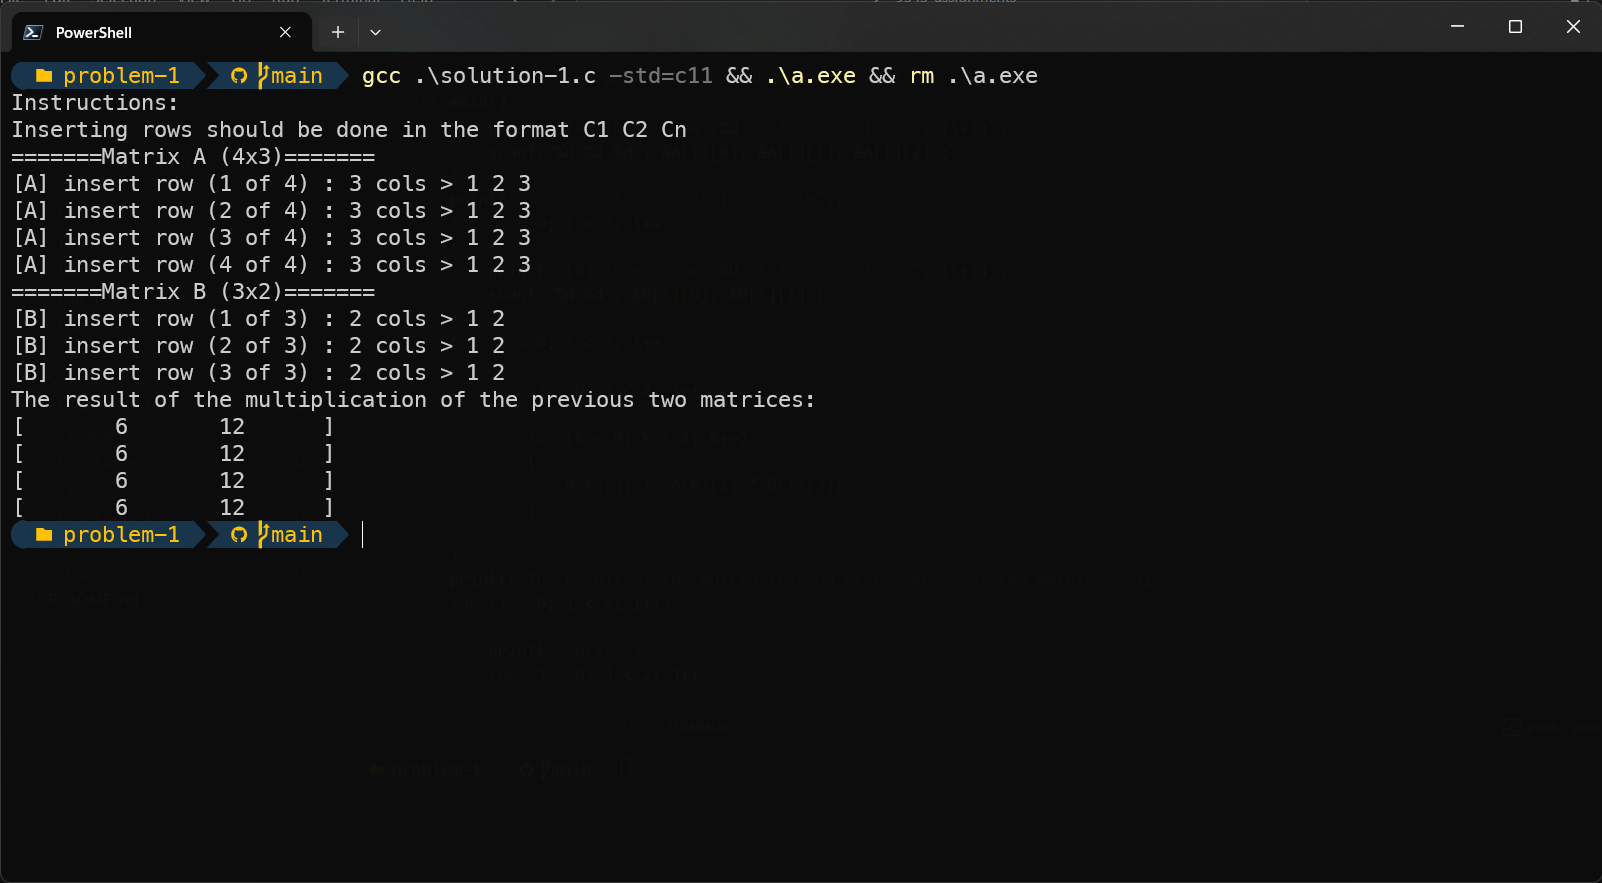
\includegraphics[width=\linewidth]{assets/prob-1.png}
    \caption{Screenshot of Problem (1)'s program input/ output}
\end{figure}
\begin{figure}[!h]
    \centering
    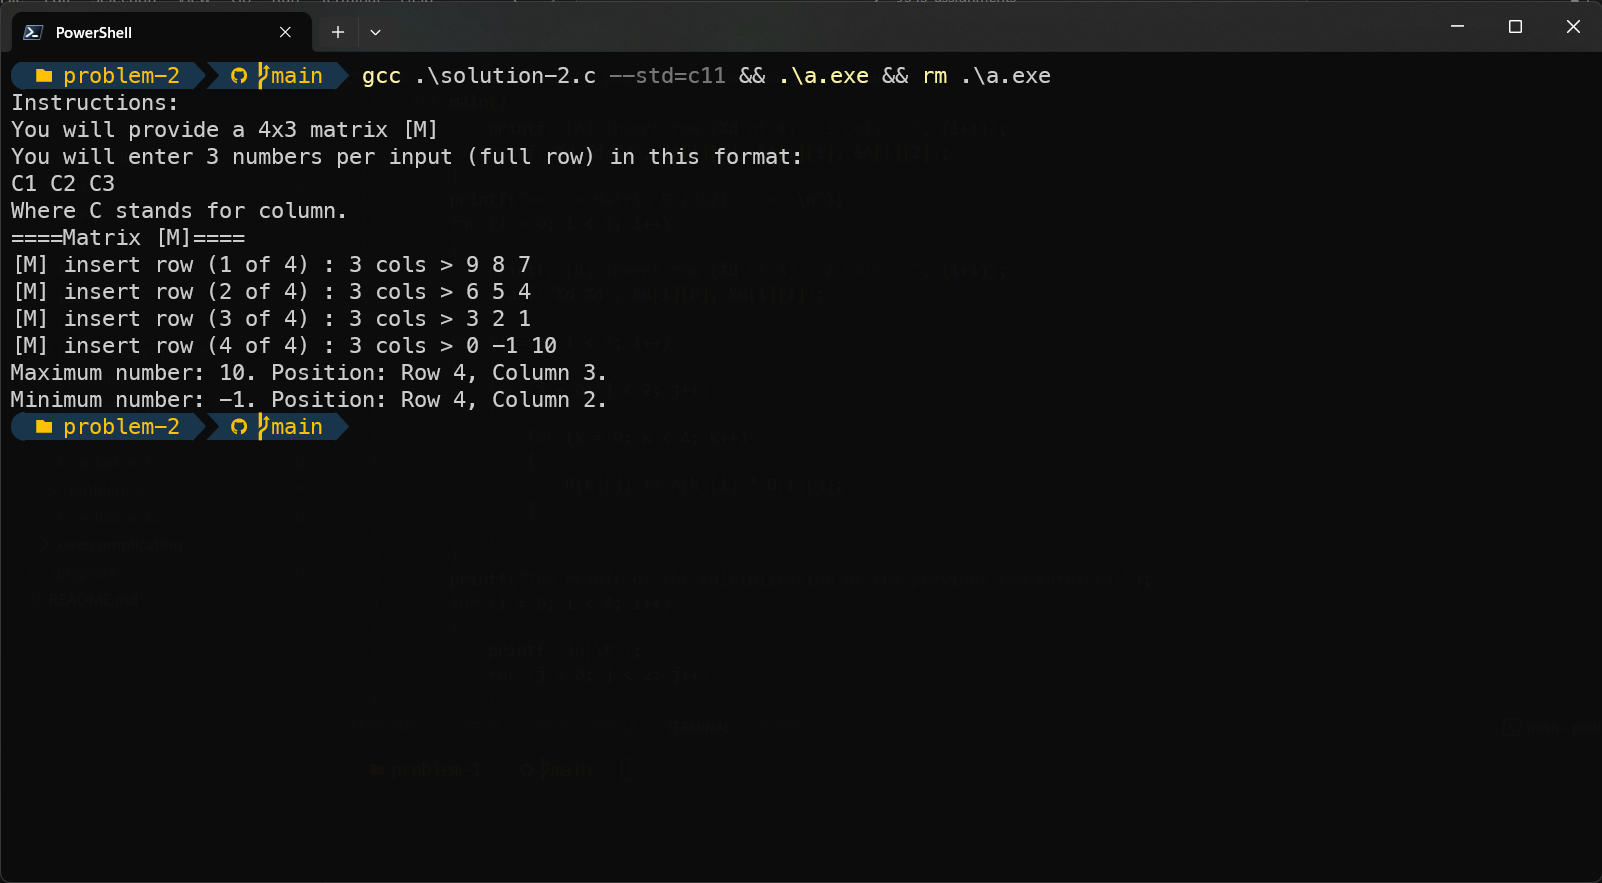
\includegraphics[width=\linewidth]{assets/prob-2.png}
    \caption{Screenshot of Problem (2)'s program input/ output}
\end{figure}
\newpage
\begin{figure}[!h]
    \centering
    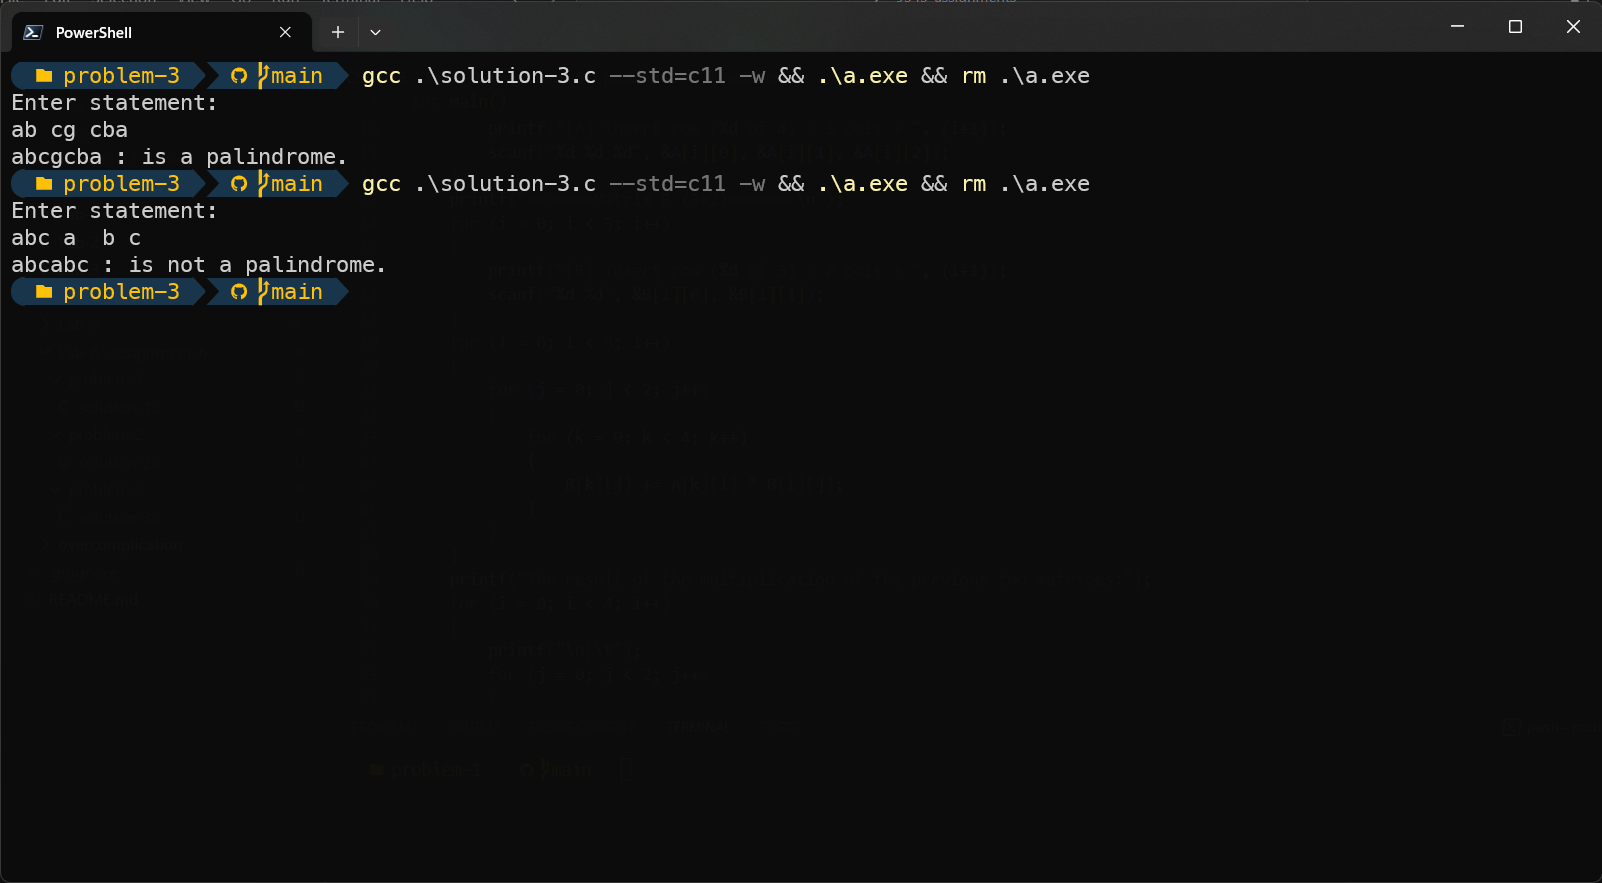
\includegraphics[width=\linewidth]{assets/prob-3.png}
    \caption{Screenshot of Problem (3)'s program input/ output (Compiler warnings suppressed)}
\end{figure}
\section{Specifications}
\begin{itemize}
    \item \textbf{Libraries:}
    \begin{itemize}
        \item \texttt{\color{inlinecode}{stdio.h}}
        \item \texttt{\color{inlinecode}{string.h}} (problem 3)
    \end{itemize}
    \item \textbf{Compiler:} GNU C Compiler \texttt{\color{inlinecode}{(gcc)}} version 13.2.0 (x86\_64-posix-seh-rev1)
    \item \textbf{C Standard Compatibility}
    \begin{center}
        \begin{tabular}{|c|c|c|c|c|c|}
             \hline
             \textbf{P\#} & \textbf{C89/C90} & \textbf{C99} & \textbf{C11} & \textbf{C17} & \textbf{C23} \\
             \hline
              1 & \checkmark & \checkmark & \checkmark & \checkmark & \checkmark \\
              2 & \checkmark & \checkmark & \checkmark & \checkmark & \checkmark \\
              3 & \checkmark & \checkmark & \checkmark & \checkmark & \checkmark \\
             \hline
        \end{tabular}
    \end{center}
    
    %\begin{flushright}
    %    \begin{tabular}{c|c}
    %         Symbol & Compatibility  \\
    %         \hline
    %         \checkmark & Full \\
    %         $\sim$ & Non-Fatal Errors \\
    %         $\times$ & Incompatible
    %    \end{tabular}
    %\end{flushright}
    \item \textbf{Supported Platforms:} OS: (any), architecture: (any)
    \item \textbf{Tested On:} Windows 11 64-bit
\end{itemize}
\section{Licenses}
This document, my additions to its \LaTeX \ source code, the software included and its \texttt{C} source code all come without warranty and are all subject to the BSD 3-Clause Open Source License:\\https://opensource.org/license/bsd-3-clause.\\

\begin{center}
    COPYRIGHT \copyright \ 2024, Youssef Ahmed Samy
\end{center}
\fancypagestyle{lastpage}
{
   \fancyhf{}
   \fancyfoot[C]{\textsl{END OF DOCUMENT}}
   \fancyfoot[L]{Assignment 6}
    \rfoot{Page \thepage \ of \pageref{LastPage}}
}
\thispagestyle{lastpage}
\end{document}
